% Makros zur Kompatibilitaet mit Onlinemodul: 
 \providecommand{\MoIl}[1][]{\mbox{}#1]\mathopen{}} 
 \providecommand{\MoIr}[1][]{#1[\mbox{}} 
 \providecommand{\MIntvlSep}{;} 
 \providecommand{\MElSetSep}{\, ; \, } 
 \begin{MAufgabe}{Lineare Betrags(un)gleichungen}{vr, 2016, MaTeX}
L\"osen Sie die Gleichung
$$
 \MDS 2\left| 4\, x - 2 \right|+2\, x - 3= 3 \left| 4\, x + 2 \right| +4\, x
$$  

\ifLsg\MLoesung

Im ersten Schritt k\"onnen die Terme au\ss{}erhalb der Betragszeichen zusammengefasst werden:

\begin{align*} 
 2\left| 4\, x - 2 \right|+2\, x - 3= 3 \left| 4\, x + 2 \right| +4\, x\\ 
\Leftrightarrow2\, \left|4\, x - 2\right| - 2\, x - 3\, \left|4\, x + 2\right| - 3= 0 
 \end{align*}

F\"ur diese Gleichung haben wir 4 F\"alle zu unterscheiden: 
\begin{enumerate}
\item $ \MDS 
\begin{cases} 
 0 \leq 4\, x - 2\\ 
0 \leq 4\, x + 2
 \end{cases}
\Leftrightarrow \frac{1}{2} \leq x\Leftrightarrow x \in [ \frac{1}{2} \, \MIntvlSep \, \infty\MoIr $ 
\item $ \MDS 
\begin{cases} 
 0 \leq 4\, x - 2\\ 
4\, x + 2 < 0
 \end{cases}
 \mbox{ : keine L\"osung. Diese Bedingung ist nirgendwo erf\"ullt.}$ 
\item $ \MDS 
\begin{cases} 
 4\, x - 2 < 0\\ 
0 \leq 4\, x + 2
 \end{cases}
\Leftrightarrow x < \frac{1}{2} \wedge - \frac{1}{2} \leq x\Leftrightarrow x \in [ - \frac{1}{2} \, \MIntvlSep \, \frac{1}{2}\MoIr $ 
\item $ \MDS 
\begin{cases} 
 4\, x - 2 < 0\\ 
4\, x + 2 < 0
 \end{cases}
\Leftrightarrow x < - \frac{1}{2}\Leftrightarrow x \in \MoIl  -\infty \, \MIntvlSep \, - \frac{1}{2}\MoIr $ 
\end{enumerate} 
Der 2. Fall ist nirgendwo erf\"ullt. Betrachte weiter nur die restlichen F\"alle.
 
 Fallunterscheidung: 

 \begin{enumerate} 
 \item Sei $ \MDS x\in[ \frac{1}{2} \, \MIntvlSep \, \infty\MoIr $. 
 In diesem Fall gilt: 
  $ \MDS \left| 4\, x - 2\right|=4\, x - 2$ und $ \MDS \left| 4\, x + 2\right|=4\, x + 2$. \\ 
 Damit ist die Gleichung 
 $$ 
2\, \left|4\, x - 2\right| - 2\, x - 3\, \left|4\, x + 2\right| - 3= 0
$$
 \"aquivalent zur Gleichung
 $$ 
2\left(4\, x - 2\right)-3\left( 4\, x + 2\right)- 2\, x-3= 0 
$$  
$$ 
 \Leftrightarrow  - 6\, x - 13= 0 
$$  
$$ \Leftrightarrow x = - \frac{13}{6} . 
 $$ 
 Die L\"osung muss auch die Fallbedingung $x\in [ \frac{1}{2} \, \MIntvlSep \, \infty\MoIr  $ erf\"ullen. Die gefundene L\"osung $x=- \frac{13}{6}$ erf\"ullt die Fallbedingung  $x\in [ \frac{1}{2} \, \MIntvlSep \, \infty\MoIr $ nicht und deshalb ist  $$
 \mathcal{L}_{1}=\emptyset 
 $$ 
\item Sei $ \MDS x\in[ - \frac{1}{2} \, \MIntvlSep \, \frac{1}{2}\MoIr $. 
 In diesem Fall gilt: 
  $ \MDS \left| 4\, x - 2\right|=2 - 4\, x$ und $ \MDS \left| 4\, x + 2\right|=4\, x + 2$. \\ 
 Damit ist die Gleichung 
 $$ 
2\, \left|4\, x - 2\right| - 2\, x - 3\, \left|4\, x + 2\right| - 3= 0
$$
 \"aquivalent zur Gleichung
 $$ 
2\left(2 - 4\, x\right)-3\left( 4\, x + 2\right)- 2\, x-3= 0 
$$  
$$ 
 \Leftrightarrow  - 22\, x - 5= 0 
$$  
$$ \Leftrightarrow x = - \frac{5}{22} . 
 $$ 
 Die L\"osung muss auch die Fallbedingung $x\in [ - \frac{1}{2} \, \MIntvlSep \, \frac{1}{2}\MoIr  $ erf\"ullen. Die gefundene L\"osung $x=- \frac{5}{22}$ erf\"ullt die Fallbedingung  $x\in [ - \frac{1}{2} \, \MIntvlSep \, \frac{1}{2}\MoIr $ und deshalb ist  $$
 \mathcal{L}_{2}=\left\{- \frac{5}{22}\right\}
 $$ 
\item Sei $ \MDS x\in\MoIl  -\infty \, \MIntvlSep \, - \frac{1}{2}\MoIr $. 
 In diesem Fall gilt: 
  $ \MDS \left| 4\, x - 2\right|=2 - 4\, x$ und $ \MDS \left| 4\, x + 2\right|= - 4\, x - 2$. \\ 
 Damit ist die Gleichung 
 $$ 
2\, \left|4\, x - 2\right| - 2\, x - 3\, \left|4\, x + 2\right| - 3= 0
$$
 \"aquivalent zur Gleichung
 $$ 
2\left(2 - 4\, x\right)-3\left(  - 4\, x - 2\right)- 2\, x-3= 0 
$$  
$$ 
 \Leftrightarrow 2\, x + 7= 0 
$$  
$$ \Leftrightarrow x = - \frac{7}{2} . 
 $$ 
 Die L\"osung muss auch die Fallbedingung $x\in \MoIl  -\infty \, \MIntvlSep \, - \frac{1}{2}\MoIr  $ erf\"ullen. Die gefundene L\"osung $x=- \frac{7}{2}$ erf\"ullt die Fallbedingung  $x\in \MoIl  -\infty \, \MIntvlSep \, - \frac{1}{2}\MoIr $ und deshalb ist  $$
 \mathcal{L}_{3}=\left\{- \frac{7}{2}\right\}
 $$ 
 \end{enumerate} 
  Die L\"osungsmenge des Ausgangsproblems ist die Vereinigung der einzelnen L\"osungsmengen: 
$$ \mathcal{L} = \mathcal{L}_{1} \cup \mathcal{L}_{2} \cup \mathcal{L}_{3} 
 = \emptyset\cup \left\{- \frac{5}{22}\right\}\cup \left\{- \frac{7}{2}\right\} 
  =\left\{- \frac{5}{22}\right\}\cup\left\{- \frac{7}{2}\right\} 
  = \left\{- \frac{5}{22}\MElSetSep- \frac{7}{2}\right\} 
 . $$ 
 
 \begin{center}
 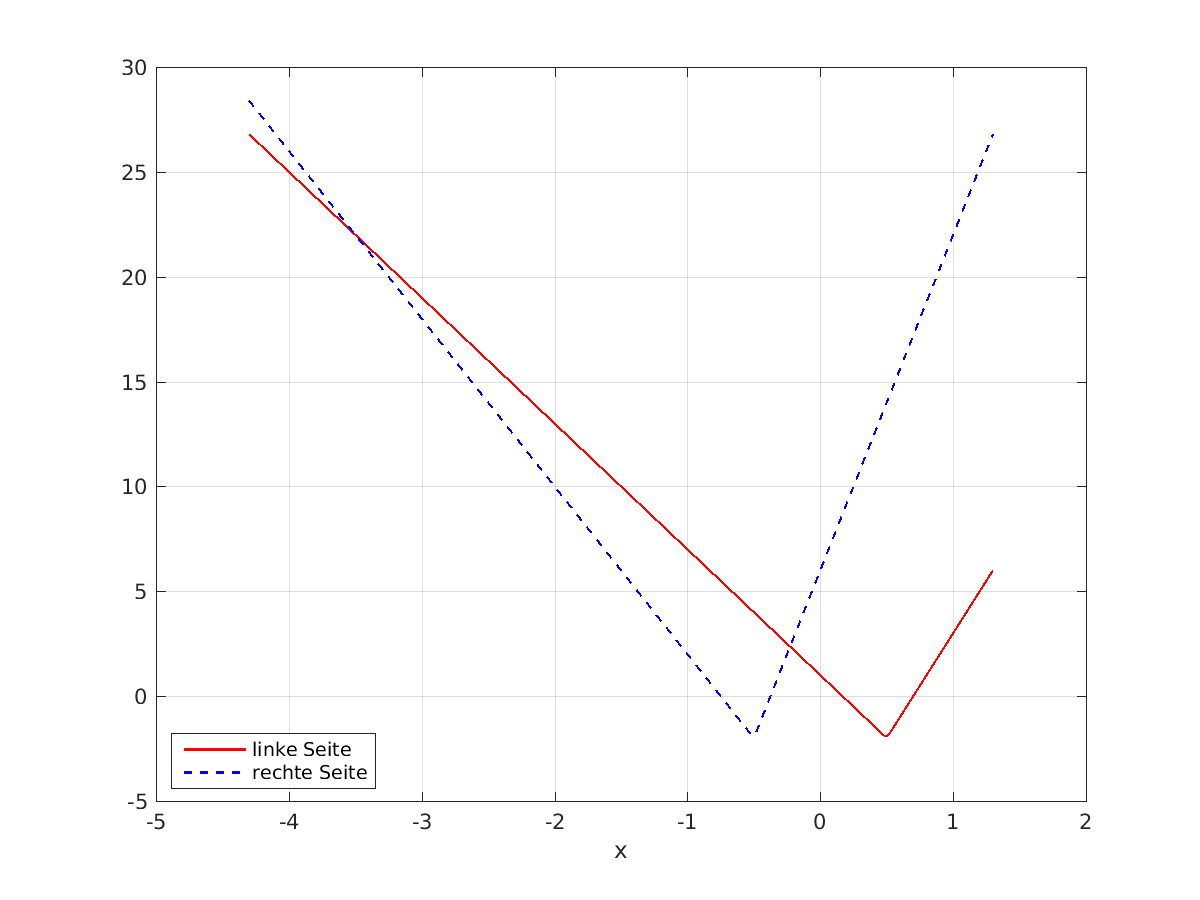
\includegraphics[width=0.8\linewidth]{Abb_zur_Ag_autogenerated_ineq_9.png} \end{center}
 
\else\relax\fi
 \end{MAufgabe}